%--
\chapter{分治递归求解}

%----------------------------------------
\section*{授课提纲}

\nid 分治策略的基本概念
\begin{itemize}
    \item 递归，作为一种思维模式；解递归方程，作为一种算法分析手段
    \item 从简单递归到分治策略
    \item 分治的典型模式（难分易合、易分难合）与样例
\end{itemize}

\nid 解递归的基本技术
\begin{itemize}
    \item 忽略取整，笨展开
    \item Guess \& Prove：一种定制版的数学归纳法
\end{itemize}

\nid 分治递归求解
\begin{itemize}
    \item 笨展开+Recursion Tree
    \item Master定理，三种情况的由来，等比数列：公比大于1、等于1、小于1
    \item Case 3的进一步解释
\end{itemize}

%----------------------------------------
\section{Master定理}

%--
\begin{theorem}[Master定理]

令$a \geq 1$和$b>1$为常数，$f(n)$为一定义于非负整数上的函数。$T(n)$为定义于非负整数上的递归函数：
%--  --
\begin{align}
    T(n) = aT\left(\frac{n}{b}\right) + f(n) \label{eqn:T(n)-1}
\end{align}
\noindent 递归式中的$\frac{n}{b}$指的是$\floor{\frac{n}{b}}$或者$\ceil{\frac{n}{b}}$。
$T(n)$的渐近增长率为：

%-- --
\begin{enumerate}[leftmargin=1em]
    \item 如果存在某个常数$\epsilon > 0$，使得$f(n) = O(n^{\log_b a - \epsilon})$，则$T(n) = \Theta(n^{\log_b a})$。
    \item 如果$f(n) = \Theta(n^{\log_b a})$，则$T(n) = \Theta(n^{\log_b a} \log n)$。
    \item 如果存在常数$\epsilon > 0$，使得$f(n) = \Omega(n^{\log_b a + \epsilon})$，且存在某个常数$c<1$，使得对所有充分大的$n$，$a f(\frac{n}{b}) \leq c f(n)$，则$T(n) = \Theta(f(n))$。
\end{enumerate}

\end{theorem}

%--
\begin{proof}

根据图\ref{f:recursion-tree}，我们有：
%--
\begin{align} \label{eqn:T(n)-2}
    T(n) &= \underbrace{\Theta(n^{\log_b a})}_{\text{叶节点层代价}} + \underbrace{g(n)}_{\text{所有非叶结点层代价}}  
\end{align}

%--
\begin{align}
    g(n) &= \sum_{j=0}^{\floor{log_b n}} a^j f(\frac{n}{b^j}) \label{eqn:g(n)}
\end{align}

\noindent 对于$g(n)$的求和形式，注意当$j$取0时，我们得到$f(n)$。
此外，求和的项数必须是整数。
\pur
递归树的层数记为$\floor{\log_b n}+1$，则非叶子节点有$\floor{\log_b n}$层，即$g(n)$的求和形式有$\floor{\log_b n}$项。
\bla

\para{第一种情况}
%
已知$f(n) = O(n^{\log_b a - \epsilon})$，所以$f(\frac{n}{b^j}) = O((\frac{n}{b^j})^{\log_b a - \epsilon})$。
据此，我们有$g(n)$满足：
%--
\begin{align*}
    g(n) &= \sum_{j=0}^{\floor{log_b n}} a^j (\frac{n}{b^j})^{\log_b a - \epsilon} \\
    &= n^{\log_b a - \epsilon} \sum_{j=0}^{\floor{log_b n}} (\frac{ab^{\epsilon}}{b^{\log_b a}})^j \\
    &= n^{\log_b a - \epsilon} \sum_{j=0}^{\floor{log_b n}} (b^{\epsilon})^j \\
    &= n^{\log_b a - \epsilon} (\frac{b^{\epsilon \log_b n}-1}{b^{\epsilon}-1}) \\
    &= n^{\log_b a - \epsilon} (\frac{n^{\epsilon -1}}{b^{\epsilon}-1})
\end{align*}

\noindent 上面的推导过程中，为了表示的方便，我们省去了$g(n)$表达式中的渐进增长率符号$O(\cdot)$。
因为$b$和$\epsilon$为常数，所以我们有$g(n) = O(n^{\log_b a - \epsilon} n^{\epsilon}) = O(n^{\log_b a})$。
所以根据公式\ref{eqn:T(n)-2}，我们证明了$T(n) = \Theta(n^{\log_b a})$。

\para{第二种情况} 
%
已知$f(n) = \Theta(n^{\log_b a})$，则$f(\frac{n}{b^j}) = \Theta( (\frac{n}{b^j})^{\log_b a} )$。
据此，我们有$g(n)$满足：
%--
\begin{align*}
    g(n) &= \sum_{j=0}^{\floor{log_b n}} a^j (\frac{n}{b^j})^{\log_b a} \\
    &= n^{\log_b a} \sum_{j=0}^{\floor{log_b n}} (\frac{a}{b^{\log_b a}})^j \\
    &= n^{\log_b a} \sum_{j=0}^{\floor{log_b n}} 1 \\
    &= n^{\log_b a} \log_b n
\end{align*}

\noindent 上面的推导过程中，为了表示的方便，我们同样省去了$g(n)$表达式中的渐进增长率符号$\Theta (\cdot)$。
根据公式\ref{eqn:T(n)-2}，我们证明了$T(n) = \Theta(n^{\log_b a} \log n)$。

\para{第三种情况} 
%
根据$T(n)$的原始表达式（公式\ref{eqn:T(n)-1}），我们知道$T(n) = \Omega(f(n))$。
所以，为了证明$T(n) = \Theta(f(n))$，我们的任务只剩下证明$T(n) = O(f(n))$。
%
根据第三种情况的第一个条件：存在常数$\epsilon > 0$，使得$f(n) = \Omega(n^{\log_b a + \epsilon})$。根据$T(n)$的递归树展开表达式（公式\ref{eqn:T(n)-2}），我们有$T(n)$的第一项$n^{\log_b a} = O(f(n))$。
此时我们的任务只剩下证明$T(n)$的第二项$g(n) = O(f(n))$。而这一结论，完全是第三种情况的第二个条件，给“硬性规定出来”的。

对于第三种情况，已知$a f(\frac{n}{b}) \leq c f(n)$，
    所以 $a^2 f(\frac{n}{b^2}) = a \cdot a f(\frac{n/b}{b}) \leq a \cdot c f(\frac{n}{b}) \leq c^2 f(n)$。
上述展开可以作用任意$j$次：$a^j f(\frac{n}{b^j}) \leq c^j f(n)$。所以根据公式\ref{eqn:g(n)}，我们有$g(n)$满足：
%--
\begin{align*}
    g(n) &= \sum_{j=0}^{\floor{log_b n}} a^j f(\frac{n}{b^j}) \\
    &\leq \sum_{j=0}^{\floor{log_b n}} c^j f(n) \\
    &\leq f(n) \sum_{j=0}^{\infty} c^j \qquad \text{($c<1$)} \\
    &= O(f(n))
\end{align*}

\noindent 由此，我们证明了$T(n) = \Theta(f(n))$
    \footnote{证明过程参考了《算法导论》的第三版和第四版的相关章节。图示基于陈道蓄老师的授课胶片修改。}
    。

\end{proof}

%--
\begin{figure}[ht]
    \center
    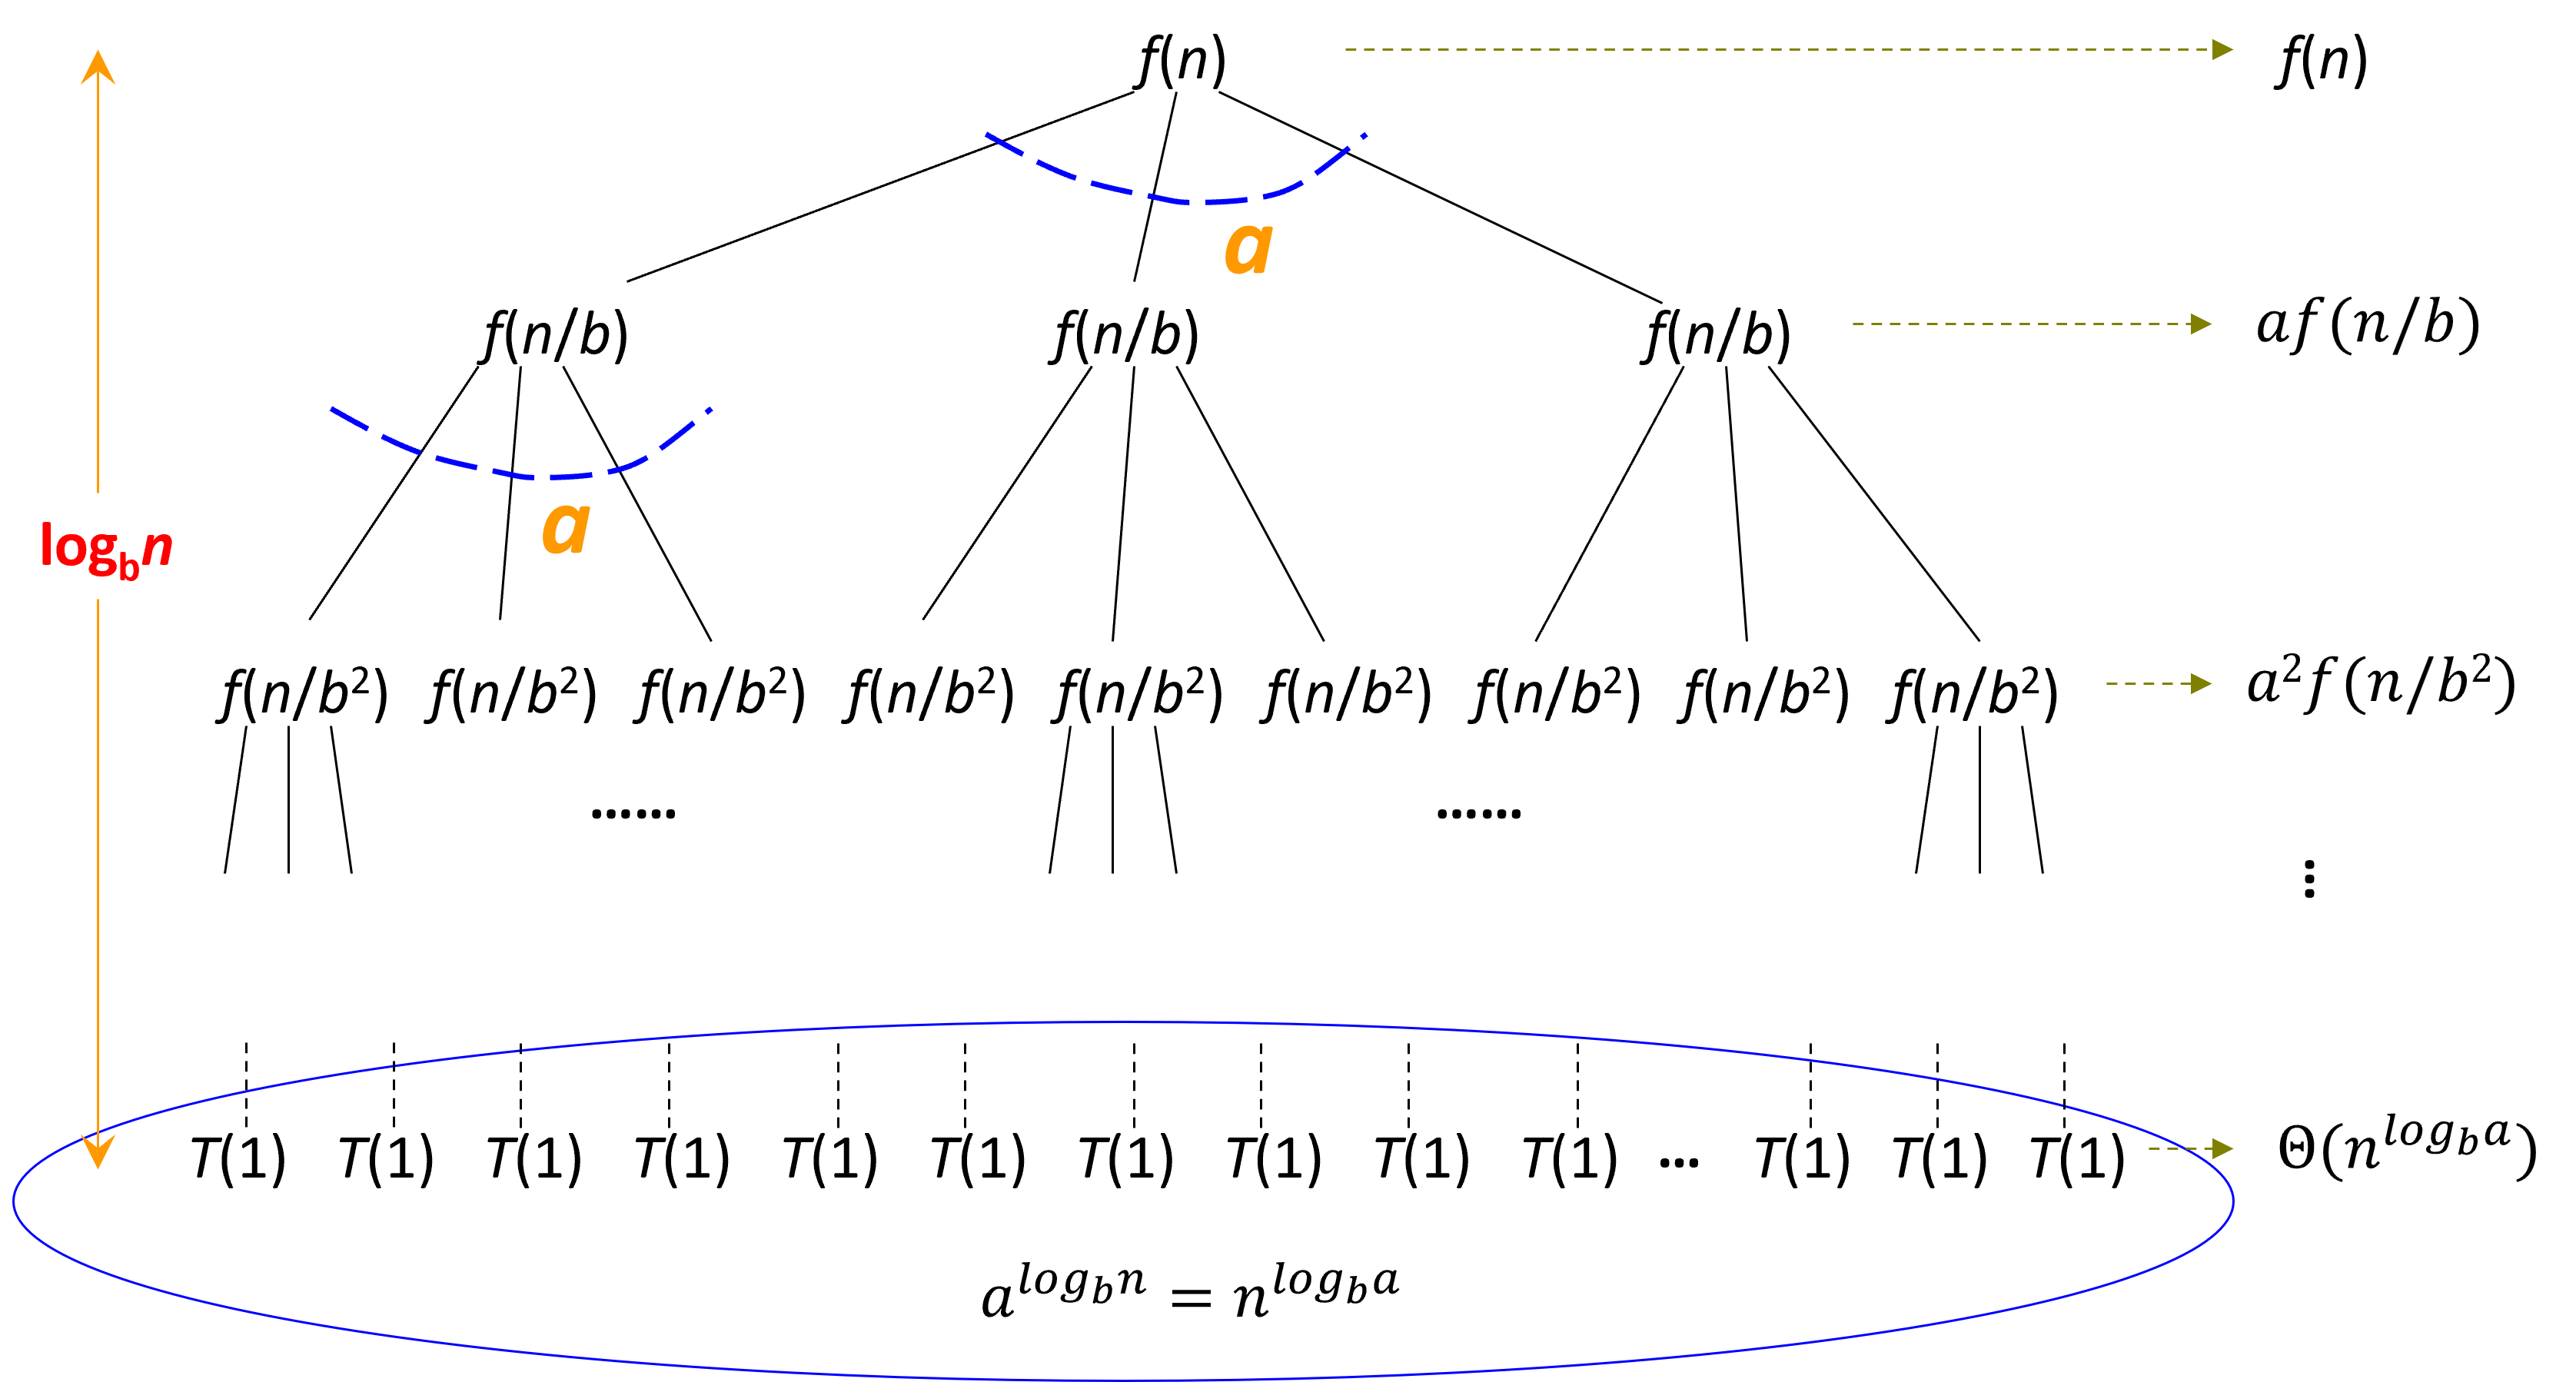
\includegraphics[width=0.75\columnwidth]{./figs/recursion/recursion-tree.png}
    \caption{$T(n)$的递归树展开}
    \label{f:recursion-tree}
\end{figure}
